% PVLDB (VLDB 2027, Vol. 20) submission, converted from the named (arXiv)
% manuscript "Paper 1 Manuscript Draft - Named (arXiv).md".
% Template: vldbproceedings/VLDB-Template (acmart.cls v2.19 + pvldb.sty).

\documentclass[sigconf, nonacm]{acmart}

%%% do not modify the following VLDB block %%
%%% VLDB block start %%%
\usepackage{pvldb}% VLDB/PVLDB formatting overrides, see pvldb.sty for details.
                      % Do not remove -- required for consistent proceedings
                      % formatting across all VLDB submissions.
%%% VLDB block end %%%

\usepackage{booktabs}
\emergencystretch=1.5em
\usepackage{fvextra}

%% The following must be set for each paper.
\renewcommand\vldbdoi{XX.XX/XXX.XX}
\renewcommand\vldbpages{XXX-XXX}
% leave empty if no availability url should be set
\renewcommand\vldbavailabilityurl{https://github.com/moganakumaran/failure-memory-text-to-sql}

\begin{document}
\title{Episodic Failure Memory Does Not Help Text-to-SQL Agents: A Compute-Fair, Corrected-Label Evaluation on BIRD [Experiment, Analysis \& Benchmark]}

\author{Mogana Kumaran Sivaraman}
\authornote{This work was conducted independently by the author and does not reflect the views of any employer.}
\affiliation{%
  \institution{Independent Researcher}
  \city{San Francisco}
  \state{CA}
  \country{USA}
}
\email{moganakumaran@ieee.org}

\keywords{Text-to-SQL, LLM agents, episodic memory, agent evaluation, benchmark label quality, compute-fair comparison, schema drift}

\begin{abstract}
Episodic memory of past failures is widely assumed to help LLM agents, and memory mechanisms are a standard component of agent architectures. We test that assumption for Text-to-SQL agents over relational databases. We use the evaluation conditions the claim actually requires: a pre-registered protocol, paired comparisons under an attempt-matched protocol with complete token accounting, and scoring against both original benchmark labels and independently audited corrected labels. On a purpose-built split of 100 recurring-failure task pairs from BIRD, episodic memory does not improve pass@1 over a no-memory baseline. The memory tested is similarity-retrieved raw episodic traces of the agent's own execution-verified, self-accepted repairs, in two variants of one retrieval design. The similarity backend (an embedding model, with a hashed term-frequency fallback) was not logged per run (\S7). The failure-fingerprinted variant, whose exact-match fast-path fired in only 9 of 400 Session-2 trajectories, scores $-1.8$ points (95\% CI $-5.7\ldots+2.1$). The generic variant scores $-4.6$ points ($-9.5\ldots0.0$). Both cost equal or greater tokens than the baseline. The null replicates exactly (0.0 points, $-4.6\ldots+4.6$) on an open-weight model, whose memory store was thin (acquisition rate 0.132; \S5.5), and holds at pass$^k$ for $k = 2$ and 4, at the resolution four runs per task afford. Under a purpose-built drift split (60 tasks, 55\% silent semantic drift), memory frozen before the drift is neutral on silent drift at this precision (point estimate 0.0 on original labels, $-5.3\ldots+4.6$, on the 33 silent tasks; $+1.5$ on the corrected view). That frozen memory is the hypothesized stale-memory hazard. A paired control on identical tasks puts the drift effect itself at $-8.3$ points on original labels ($-18.3\ldots+1.7$) and $-8.3$ points on corrected labels ($-17.5\ldots+0.4$), the corrected view scored against drift-adjusted corrected golds. Neither interval excludes zero at $n = 60$. The study's one positive arm is diagnostic rather than decisive. Generate-and-select beats no-memory by $+9.8$ points on original labels but by exactly 0.0 on corrected labels, while running 17\% over its nominal token budget. The two contrasts use different task sets (97 vs 49 tasks); on the 49 corrected-label tasks alone, the original-label margin is $+10.2$, so the collapse is produced by the label change on identical tasks, not by the subset change. This is consistent with label noise and loose compute accounting jointly producing an apparent win, though the corrected subset (49 tasks, $\pm$8 points) cannot by itself exclude a real effect. Under a strictly enforced cap in the replication, the same arm is null on original labels as well. A post-hoc verifier ablation (Amendment A14, extended by the A15 store transplant) adds a further caution: the base agent's self-verifier is a net harm ($-8.5$ to $-9.8$ points), and the memory null persists without it, including when the verifier-off agent is given a full-size transplanted memory store (\S5.6). We release the evaluation design, the drift split construction, and a strict no-gold memory-acquisition methodology (56.5\% acquisition rate) as reusable artifacts. Our conclusion is narrow and, we argue, useful. On this substrate, under attempt-matched comparison, episodic failure memory of the form we test is not where the gains are. Evaluations that do not control labels and tokens cannot be trusted to say where they are.
\end{abstract}

\maketitle

%%% do not modify the following VLDB block %%
%%% VLDB block start %%%
\vldbtopmatter
%%% VLDB block end %%%

\section{Introduction}

Agent memory is having its framework moment. Long-term episodic stores, reflection buffers, and failure libraries are built into most serious agent stacks. The intuition behind them is appealing: an agent that has seen a failure before should not repeat it. For data agents, the intuition seems especially strong. Data agents are systems that answer questions by generating and executing SQL over enterprise schemas. Failures recur: the same schema quirks, value formats, and join traps appear across questions on the same database.

Yet the evidence base for failure memory in data work is thin in a specific way. The highest BIRD execution accuracy reported by a multi-agent Text-to-SQL system at its time, CHASE-SQL (73.01\% dev, 73.0\% test), is a generate-and-select method whose gains come at explicitly higher test-time compute; it says nothing about memory. General-domain agent research offers a cautionary signal. Consolidated LLM memory has been shown to degrade performance below a no-memory baseline in some settings. Recent work on stale retrieval and silent environment change shows memory hurting agents in ways retrieval metrics do not detect. But no published study, to our knowledge, tests failure memory for data agents with compute accounting against audited labels. Meanwhile the labels themselves are suspect. A recent audit of BIRD and Spider 2.0 reported a 52.8\% annotation error rate on the BIRD Mini-Dev subset it audited, with leaderboard rank shifts of up to nine places after correction. An evaluation that ignores both problems (uncontrolled compute and noisy labels) can produce wins that do not exist.

This paper is the report of a pre-registered attempt to find out whether failure memory helps, designed so that a negative answer would be as informative as a positive one. Our protocol, hypotheses, exclusion rules, and go/no-go margins were frozen before any run and amended only through dated amendments. The answer is no. It holds across both variants of the episodic-retrieval design we test, a drift condition, a verifier ablation, and an open-model replication. The study's one positive arm turns out to be an object lesson in why the controls mattered.

\textbf{Contributions.}
\begin{enumerate}
\item \textbf{A pre-registered, attempt-matched, token-accounted test of episodic failure memory for Text-to-SQL agents.} One episodic-retrieval design in two variants (failure-fingerprinted and generic), a no-memory baseline, and a generate-and-select arm are compared pairwise on identical task pairs with paired bootstrap intervals, under an attempt-matched protocol with measured token budgets. A verifier ablation and a store-transplant condition, both post-hoc amendment analyses (A14/A15), show the base agent's self-verifier is a net harm and that the memory null is not a verifier artifact.
\item \textbf{Dual-label evaluation as a first-class control.} Every contrast is reported on original BIRD labels and on the corrected labels of Jin et al.'s audit~\cite{jin} (498 tasks). The study's headline methodological finding is only visible because both views were pre-committed. That finding is a $+9.8$-point effect on original labels that does not survive corrected labels (0.0 points, $\pm$8; at 17\% over its token cap; \S5.2). On the 49 corrected-label tasks alone, the original-label effect is $+10.2$, so the non-survival is a label effect on identical tasks, not a subset effect.
\item \textbf{A drift split for data agents, a paired drift measurement, and a stale-memory test.} Sixty execution-verified drifted database variants (55\% silent semantic drift), a same-task undrifted control, and a frozen pre-drift memory arm let us measure both the drift effect and negative transfer directly. Drift costs about 8 points on both label views; stale memory is neutral.
\item \textbf{A strict memory-acquisition methodology.} Memory episodes are acquired only from agent-discovered, execution-verified remediations. Gold SQL never touches the store. The acquisition rate (56.5\%) is reported as a headline statistic, so a null result cannot be dismissed as an empty store.
\end{enumerate}

\section{Related work}

\textbf{Benchmarks and the label problem.} BIRD~\cite{bird} is the standard large-scale Text-to-SQL benchmark: 12,751 question--SQL pairs over 95 databases, where GPT-4 reached 54.89\% execution accuracy against 92.96\% human performance. Spider 2.0~\cite{spider2} moves to enterprise workflows, where a leading agent scored 17.0\% (arXiv v1) to 21.3\% (ICLR 2025 version). Version matters when quoting results. Jin et al.~\cite{jin} audited both benchmarks and reported an annotation error rate of 52.8\% on the BIRD Mini-Dev subset they audited, with corrected-label rank shifts of $-9$ to $+9$ places. Their released corrections cover 498 BIRD Dev tasks, which is the set our corrected-label view uses (\S3.1). Two recent audits reinforce the point from other angles. Retrieval metrics can rank memory policies backwards when stored facts go stale (Murshed, 2026, preprint)~\cite{stalebench}. A task-level audit of eight frontier benchmarks found verified task validity of only 29.3\% for multi-step suites against 92.5\% for closed-form benchmarks (Zhu and Cat, 2026, preprint)~\cite{benchmarks}. Label and metric validity is a live methodological problem, not a niche concern of this study.

\textbf{Data agents.} Multi-agent Text-to-SQL is an active design space. CHASE-SQL~\cite{chase} reported the highest BIRD execution accuracy among multi-agent systems at its time (73.01\% dev, 73.0\% test). It achieved this by generating diverse candidates and selecting among them at additional test-time compute. Our A3 arm mirrors that design under a budget cap. Earlier multi-agent systems include MAC-SQL~\cite{macsql} (COLING 2025; Selector/Decomposer/Refiner; 59.39\% dev in the paper, 57.56\% on the official leaderboard; we note the discrepancy) and MAG-SQL~\cite{magsql} (61.08\% on BIRD with GPT-4). They also include CHESS~\cite{chess} (dev $\approx$65--68\%, test $\approx$67--71\% depending on configuration). DIN-SQL~\cite{dinsql} (NeurIPS 2023) reaches 50.72\% dev with a single model under decomposed prompting. Decomposition gains are not inherently multi-agent. None of these systems uses cross-session failure memory; their gains, where real, come from within-task compute. SQLAgent~\cite{sqlagent} takes a different route, learning to explore the database before generating SQL; exploration targets the schema-grounding failures in our error taxonomy (\S3.5). Broader data-analysis benchmarks report best-agent accuracies of 34.12\% (DSBench~\cite{dsbench}) and 57\% (DataAgentBench~\cite{dataagentbench}, a 2026 preprint); DABstep~\cite{dabstep} (preprint) reports 14.55\% on its hardest tier, underscoring how unsettled data-agent evaluation remains.

\textbf{Agent memory.} The canonical memory mechanisms are general-domain. Reflexion~\cite{reflexion} stores verbal self-reflections in an episodic buffer and reuses them across trials. ExpeL~\cite{expel} pools raw trajectories and distils cross-task insights for recall at inference. Generative Agents~\cite{generativeagents} maintain a memory stream with reflection synthesis. MemGPT~\cite{memgpt} popularized tiered, OS-style memory. None of these was evaluated on Text-to-SQL or any data-agent task. Evidence that memory helps is mixed even in general domains. Zhang et al.~\cite{zhangmemory} show that \emph{consolidated} LLM memory degrades with repeated updating and can fall below a no-memory baseline. An episodic-only control retaining raw trajectories remains competitive. A newer line of work treats memory as a liability surface. It covers stale retrieval that standard metrics score as correct (Murshed, 2026, preprint)~\cite{stalebench}, silent environment change under which experienced agents fail where novices succeed (Xu et al., 2026, preprint)~\cite{experiencerot}, and ``memory-induced degradation'' from following wrong stored lessons (Lee et al., 2026, preprint)~\cite{wikitrace}. Our A1/A2 arms implement one form of the episodic family: verbatim replay of raw traces of the agent's own execution-verified, self-accepted repairs, with no LLM consolidation and no distillation into lessons. The null we report is a statement about that episodic-replay form. It is not a test of the abstracted variants above. Reflexion's stored unit is a verbal reflection, ExpeL's is a distilled cross-task insight, and consolidated stores rewrite their contents over time. Those are different representations, and our design cannot speak to them. Whether raw episodic memory helps \emph{data} agents was, to our knowledge, untested before this study. The gap analysis underlying it (two scoped passes over arXiv and major venues, November 2026) found the cell empty.

\textbf{Reliability measurement.} $\tau$-bench~\cite{taubench} introduced pass$^k$ as a reliability metric for agents. Pass$^k$ is the probability that all $k$ independent runs succeed. It showed steep degradation (GPT-4o below 25\% at pass$^8$ in retail). Our frozen claim was stated in pass$^k$ terms; the study's pre-committed gate used run-mean pass@1, and \S5.7 reports pass$^k$ for the primary contrasts. Failure taxonomies for multi-agent systems (e.g., MAST~\cite{mast}) are general-domain; our taxonomy (\S3.5) is derived blind from data-agent traces.

\section{Method}

\subsection{Substrate and label policy}

The substrate is classic BIRD Dev (dev\_20240627, pinned): 1,534 tasks over 11 databases. Because label quality is a variable in this study, every task carries a label status: \textbf{L1} corrected label available from Jin et al.'s audit~\cite{jin} (498 tasks; 220 with SQL differing from the original gold); \textbf{L2} original label only (1,035 tasks); \textbf{L3} disputed, no correction --- excluded from all primary metrics and logged (1 task: question 1006, a gold error discovered by this study's dry runs, in which the gold's string-parsing ordering returns a 2:00.000 lap as ``fastest'' while the milliseconds column's minimum is 1:07.411; verified by direct execution and corroborated by two independent models); \textbf{L4} ambiguous --- more than one defensible correct answer, with no corrected gold resolving it (0 tasks met this criterion; the tier was defined before the study and never used). All results are reported dually, on original labels for the full primary set and on corrected labels for the L1 subset. The manifest, splits, and all file hashes were frozen before the study. The single post-freeze change (the L3 relabelling of q1006) was made by dated amendment, with the original hash preserved. Within the corrected-label subsets used below, 20 of the 49 primary tasks have golds that differ from the original (29 are audited-unchanged), and 26 of the 60 drift tasks have differing golds. A dilution caveat applies to those counts. Across the two splits, 15 of the 46 distinct changed-gold tasks have corrected SQL that differs textually from the original but returns identical results on the undrifted database. For those tasks the two label views coincide on undrifted data, so the result-changing subsets are smaller than the counts suggest (15 primary tasks, 16 drift tasks).

\subsection{Splits}

\textbf{Repeated-failure split.} One hundred Session-1/Session-2 task pairs, clustered by database and identical table-set signature, balanced 9--10 pairs per database. Pair similarity is a structural distance, $1 - [0.5 \cdot \mathrm{Jaccard}(\text{table sets}) + 0.3 \cdot \mathrm{Jaccard}(\text{SQL skeleton tokens}) + 0.2 \cdot \mathrm{Jaccard}(\text{question tokens})]$. Observed distances run 0.086--0.307 (median 0.209). All pairs are structurally similar recurrences, spanning a band from near to moderate similarity rather than a similar/dissimilar contrast. Pairs below distance 0.10 (3 pairs) are flagged recall-control and excluded from the primary metric, leaving 97 primary Session-2 tasks; results are also stratified by distance tertile. Session 1 is where memory is acquired; Session 2 is where it is tested. Memory for a task comes only from strictly earlier sessions; Session-2 acquisitions are written to a shadow store that is counted but never retrieved within the study. A violation invalidates the run (none occurred). Two scoping notes apply to the word ``recurring'' throughout. The pairing is structural: 0.3 of the similarity weight rests on the gold queries' SQL skeletons, so gold enters split construction (it never enters the system, \S3.4), and the split tests structurally similar task pairs. We did not measure whether paired Session-1 and Session-2 tasks share failure classes at above-chance rates, so failure recurrence itself is the design's premise, not a measured property of the split.

\textbf{Drift split.} Sixty tasks, all L1, each have a drifted copy of their database. Each copy was built by one of seven operators: column rename 23, value recode 10, category merge 9, unit change 9, type change 4, temporal grain 4, null semantics 1. Thirty-three variants (55\%) are \emph{silent} (the meaning changes under unchanged column names), and 27 are overt variants, which serve as the control condition. Every variant was verified by execution before freezing. Figure~\ref{fig:drift} shows the composition by operator. Scoring on the original-label view uses the drift-adjusted original gold executed on the drifted database. Scoring on the corrected-label view uses Jin et al.'s corrected SQL~\cite{jin} after applying the same drift operator transformation that produced the drifted database: column renames, value recodes, and category merges are applied to the corrected query text, and the remaining operators leave the query unchanged. Each adjusted corrected gold was validated by execution: all 60 execute on their drifted databases. For the 23 rename tasks, the adjusted gold's result on the drifted database reproduces the corrected gold's result on the original database exactly. For the remaining operators, the corrected query text is unchanged or its value literals are adjusted to the drifted encoding, so its result reflects the drifted semantics by construction. The adjustment is not optional. Unadjusted corrected golds do not execute at all on renamed schemas (22 of the 23 rename tasks), so an unadjusted corrected view under drift is mechanically broken rather than merely approximate. \S5.4 reports the adjusted view and quantifies what the unadjusted one did.

\begin{figure}
  \centering
  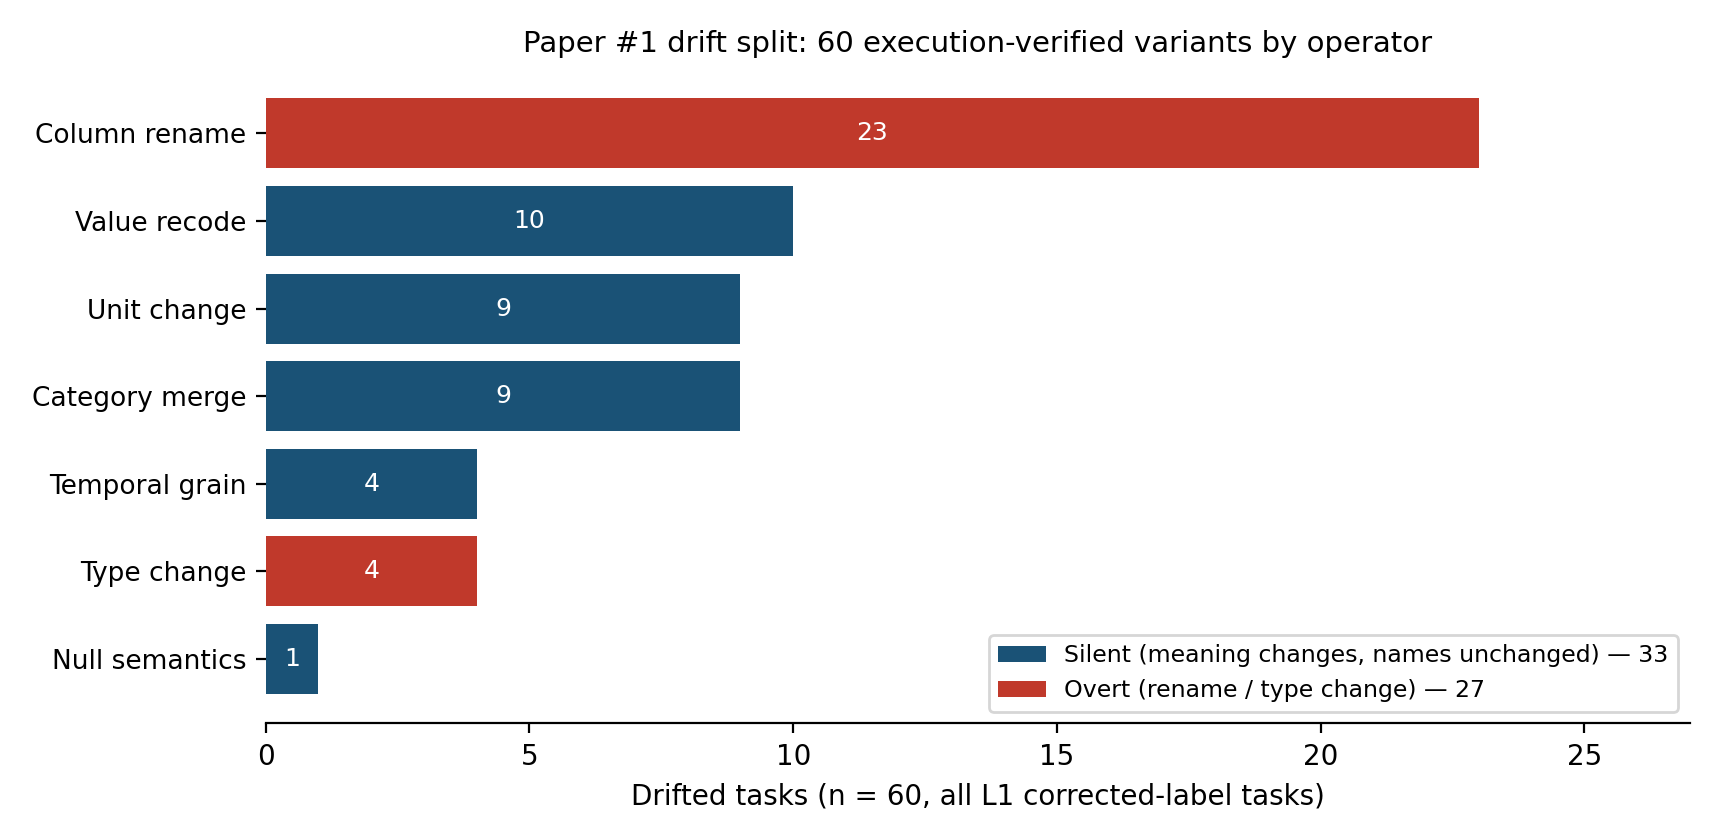
\includegraphics[width=\linewidth]{figures/fig1-drift.png}
  \caption{Drift-split composition: 60 execution-verified variants by operator, split into silent (33) and overt (27).}
  \Description{A horizontal bar chart of the 60 drifted database variants by operator: column rename 23 (overt), value recode 10, unit change 9, category merge 9, temporal grain 4, null semantics 1 (silent), and type change 4 (overt); silent variants total 33 and overt variants 27.}
  \label{fig:drift}
\end{figure}

\subsection{Arms}

All arms share one base agent: schema + evidence + question $\rightarrow$ SQL generation, read-only execution with a 10-second limit, and retry on execution error with the error fed back (maximum 3 attempts). The base agent also has a self-verification step, in which the agent's own verifier accepts or revises the result. Prompts, tools, sandbox, and step limits are identical across arms; only the memory/selection mechanism varies. (The verifier itself is ablated in \S5.6.)

\begin{itemize}
\item \textbf{A0 --- no memory.} The base agent, stateless across sessions.
\item \textbf{A1 --- failure-fingerprinted episodic memory.} Episodes are raw traces keyed by a deterministic fingerprint over (failure class, error signature, schema elements, schema version). Retrieval is exact fingerprint match, else top-$k$ ($k \leq 3$) similarity retrieval over raw traces. No LLM consolidation is applied to stored episodes. Similarity scores are produced locally (embeddings from a Qwen2.5-Coder-3B model served via Ollama, with a hashed term-frequency fallback in the harness). \S7 discloses a logging gap in which backend served the study runs.
\item \textbf{A2 --- generic episodic memory.} The same store and retrieval budget without fingerprint keying (similarity retrieval only, under the same backend arrangement as A1). \S5.3 reports how the two variants actually differed in behavior.
\item \textbf{A3 --- generate-and-select.} Three candidates are generated and executed; a selector call picks among those that executed, in the style of CHASE-SQL~\cite{chase}. Its token budget is capped at A1's measured average tokens per task (3,506). \S5.2 reports how that cap behaved as implemented. \S5.5 reports the fix applied in the replication.
\item \textbf{A4 --- stale memory (drift split only).} A1's mechanism with the store built on the original databases before drift (16--22 episodes per run), frozen at the drift boundary, and never updated during the drift phase. A1's drift-phase store, by contrast, starts empty and grows during the phase (72 episodes acquired).
\end{itemize}

\subsection{Memory acquisition policy}

The acquisition rule is the methodological core of the study, because a memory evaluation is only meaningful if the memory could plausibly have been built in deployment. An episode enters the store \textbf{only} when the agent itself recovers from a failure during a task (an execution error or a verifier rejection). The remediation is then verified by execution and accepted by the agent's own verifier. ``Verified'' in this paper means exactly that conjunction: the remediation executed, and the agent's own verifier accepted it. It never means checked against gold; episode correctness was not measured (\S7). Gold SQL, gold labels, and human fixes never create, complete, or repair an episode. Failures the agent cannot resolve go to a separate unresolved log. The \textbf{acquisition rate} is episodes acquired divided by failures the agent observed. It is reported as a headline statistic alongside accuracy, so that a null accuracy result can be checked against the possibility that the store was simply empty. The rule is enforced in harness code, not by convention.

\subsection{Failure taxonomy}

Failure classes were derived by blind open coding of dry-run traces (two annotators, 6/6 per-task primary-defect agreement on the local-model run; seed classes admitted only at reconciliation), then frozen before the study: F1 wrong schema link, F2 stale schema assumption, F3 wrong join/fan-out, F4 aggregation/grouping incl.\ temporal-snapshot semantics, F5 value-format mishandling, F6 unrecovered execution error, F7 correct content in the wrong answer shape, F8 unsafe/destructive (log-only), F9 no-change repair loop (a new class from open coding: the agent resubmits byte-identical SQL after error feedback --- observed in 8 of 8 retries of a 3B local model, absent at frontier scale). Gold-label errors are not failure classes; they are handled by the label policy in \S3.1.

\section{Experimental setup}

\textbf{Pre-registration and power.} The protocol (claim, arms, splits, exclusion rules, analysis plan) was frozen before any run. It changed afterwards only through dated amendments (A1--A15), which are released with the study artifacts. A simulation-based power analysis used dry-run base rates (per-task latent success probabilities, 4 runs per task per arm, paired test on run-mean pass@1). It found power nearly invariant to base rate in [0.30, 0.55]. The minimum detectable effect at 80\% power was 10--12 points at $n = 100$. The pre-committed GO margin for the memory hypothesis was therefore $+12$ points of paired pass@1 (A1 $-$ A0), with the 95\% CI excluding zero. The protocol also pre-committed that a null would pivot this paper to the attempt-matched negative-result framing, rather than quietly change the claim. The pre-registered primary analysis is the repeated-split contrast set of \S5.1--\S5.3. Two later additions are post-hoc and are labelled where they appear: the Amendment A14 control and ablation runs (the drift control and the verifier ablation), prompted by external critique of a draft, and the Amendment A15 store-transplant condition (\S5.6), added in revision. Neither changes the frozen primary contrasts.

\textbf{Model and harness.} The main study uses a single pinned snapshot, gpt-5-mini-2025-08-07, via API; \S5.5 replicates the primary contrasts on Qwen2.5-Coder-32B-Instruct. Four runs per task per arm throughout. Decoding was fixed by the harness's request construction, which is released with the artifacts. Main-study requests contained only the model identifier, a single user-turn message, and a completion-token cap (\texttt{max\_completion\_tokens} = 4000). No temperature or other sampling parameter was sent, so the provider's default sampling for the snapshot applied; the harness did not record it further. Replication requests, sent through OpenRouter, were constructed the same way except that they set temperature to 0 in the request body. Scoring is execution accuracy under our own scorer (released as \texttt{results\_equal} in \texttt{pilot\_lib.py}); it is not the official BIRD evaluation script. Predicted and gold SQL are each executed read-only against the task's database under the same 10-second limit, with result sets fetched up to 100,000 rows. A prediction that errors, times out, or is absent scores incorrect. A gold execution that errors or times out likewise makes the comparison false for every arm. The comparison first converts every cell value to its string representation. Column names are never compared; column order matters only through row position. If the gold query contains ORDER BY, the two stringified row lists must be identical in order. Otherwise they are compared as multisets (sorted row tuples), so duplicate rows count with multiplicity. There is no numeric tolerance: values must match exactly after string conversion, so 1 and 1.0 differ, and dates and timestamps compare as their stored strings. NULLs pass through the same string conversion on both sides. The full prompt set, including the verifier prompt, is released with the artifacts (Appendix~A). Total cost of the main study was \$14.91 across 3,760 trajectories (2,800 repeated-split, 960 drift). The replication cost \$2.37. The post-critique control and ablation runs (Amendment A14) cost \$2.81. The Amendment A15 transplant condition cost \$0.55. All were inside pre-set budget caps recorded in the amendments.

\textbf{Analysis.} The pre-registered primary contrast is A1 $-$ A0 on the repeated-failure split; all other contrasts are secondary and reported with the same paired machinery so the reader can judge multiplicity directly. The primary estimand is the paired difference in run-mean pass@1 against original BIRD golds on the 97 primary tasks. The corrected-label view is a pre-committed secondary view of the same contrasts on the 49-task L1 subset. The original-label view is primary for a practical reason: corrected labels cover only 49 of the 97 primary tasks, and the GO margin was powered on the full set. Primary contrasts are paired per-task differences in run-mean pass@1 with task-level bootstrap 95\% CIs (10,000 resamples, fixed seed). Token fairness is reported dually: attempt-matched (same step limits) and token-measured (actual mean tokens per trajectory per arm), with token-matching treated openly as an approximation.

\section{Results}

Figure~\ref{fig:forest} summarizes the main study's and replication's primary contrasts by split and label view. The subsections below give all numbers in full, including the Amendment A14 control and ablation runs and the Amendment A15 transplant condition.

\begin{figure*}[t]
  \centering
  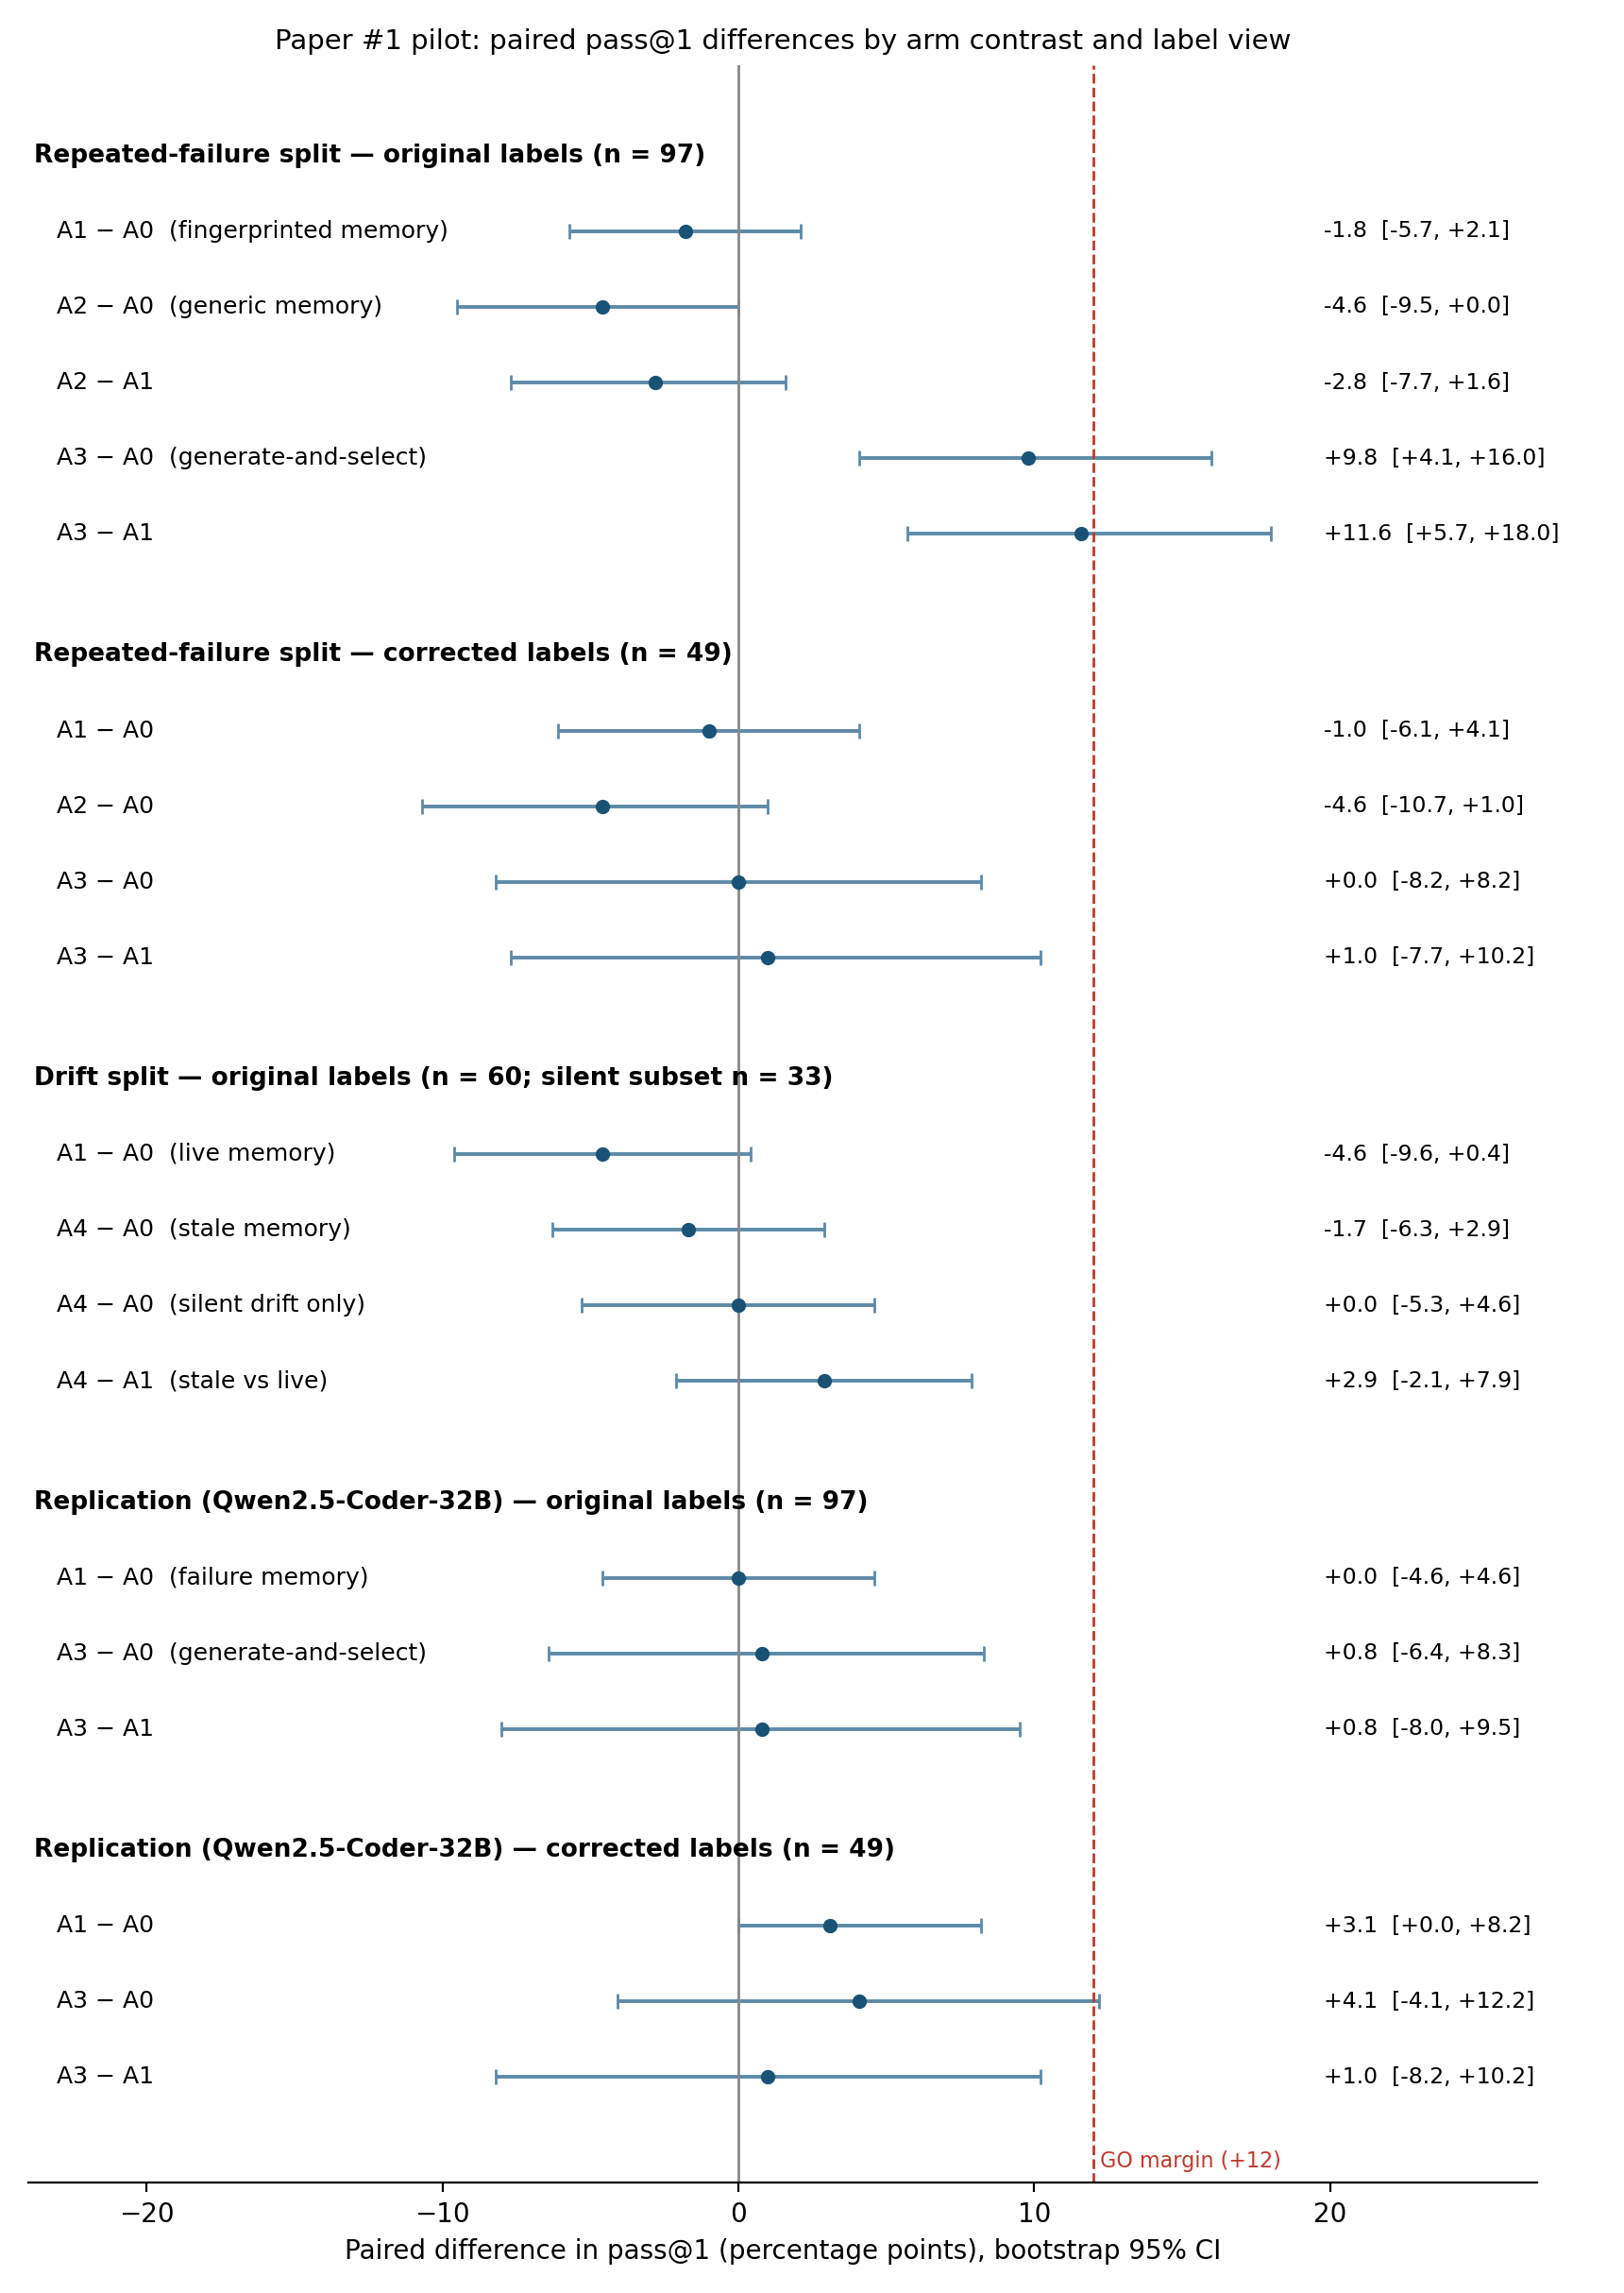
\includegraphics[width=\textwidth,height=0.82\textheight,keepaspectratio]{figures/fig2-forest.png}
  \caption{Paired pass@1 differences (percentage points) with bootstrap 95\% CIs. The contrasts cover the repeated-failure split (original and corrected labels), the drift split, and the Qwen2.5-Coder-32B replication (original and corrected labels). The dashed line marks the pre-committed $+12$-point GO margin.}
  \Description{A forest plot of paired pass@1 differences with 95\% confidence intervals, grouped by split and label view. The groups are the repeated-failure split on original and corrected labels, the drift split on original labels, and the Qwen2.5-Coder-32B replication on original and corrected labels. Nearly all intervals cross zero. The only clearly positive contrasts are A3 against A0 and A1 on original labels in the main study. A dashed line marks the pre-committed $+12$-point GO margin.}
  \label{fig:forest}
\end{figure*}

\subsection{Failure memory does not help (primary contrast)}

On the 97 primary Session-2 tasks, the no-memory baseline A0 scores 0.539 pass@1. Failure-fingerprinted memory (A1) scores 0.521: a paired difference of \textbf{$-1.8$ points (95\% CI $-5.7\ldots+2.1$)}. The pre-committed GO criterion ($+12$ points, CI excluding zero) fails by a wide margin. The interval rules out any true gain larger than $\approx$2 points in this regime. This is an informative null, not merely an underpowered one. On the 49 primary tasks with corrected labels the difference is $-1.0$ points ($-6.1\ldots+4.1$). Restricting the corrected view to the 20 tasks whose golds actually changed leaves the contrast materially unchanged ($-1.3$ points, $-8.8\ldots+6.3$). The corrected-label null is therefore not a dilution artifact of the 29 audited-unchanged tasks. Stratified by pair-distance tertile, no stratum is significantly positive (near $-3.8$, mid $+0.8$, far $-2.3$ points, all intervals spanning zero). The null is not hiding among the most similar task pairs.

The store was not empty. In Session 1, A1 observed 177 failures and acquired \textbf{100 execution-verified episodes (acquisition rate 0.565)} under the no-gold policy of \S3.4; 77 failures were unresolved and logged. A1's Session-2 trajectories used a mean of 3,506 tokens against A0's 2,862 ($+22\%$, the injected memory context) at essentially identical attempt counts (1.69 vs 1.68). Memory cost more compute and returned nothing.

\subsection{Generate-and-select: a label-dependent win, over budget}

A3 is the study's only positive arm on original labels: 0.637 pass@1. It beats A0 by \textbf{$+9.8$ points ($+4.1\ldots+16.0$)} and A1 by \textbf{$+11.6$ ($+5.7\ldots+18.0$)}. On the 49 corrected-label tasks, however, both differences collapse --- \textbf{0.0 points vs A0 ($-8.2\ldots+8.2$)} and $+1.0$ vs A1 ($-7.7\ldots+10.2$). The two headline contrasts use different task sets, so we also computed the original-label contrasts on the identical 49 tasks, from the stored traces. On those tasks A3 scores 0.582 against A0's 0.480, a margin of $+10.2$ points ($+1.5\ldots+19.9$), and $+11.2$ against A1 ($+2.0\ldots+21.4$). Restricting the task set therefore does not shrink the win. The collapse happens when the labels change on the same tasks, which excludes subset composition as its explanation. Two readings of the corrected-label null itself remain live. In the first, the original-label win is a label-noise artifact (generate-and-select is better at matching buggy golds). In the second, the 49-task corrected view is underpowered ($\pm$8 points) and cannot exclude a real effect. The corrected view cannot distinguish these, and we report both rather than claim the win. The replication (\S5.5) adds one supporting leg for the artifact reading: under a strictly enforced token cap, A3 is null on original labels too. The changed-gold sensitivity analysis leans the same way without settling it. On the 20 tasks whose golds actually changed, the corrected A3$-$A0 contrast is $-7.5$ points ($-18.8\ldots+1.3$). On the 29 audited-unchanged tasks it is $+5.2$ ($-5.2\ldots+16.4$). A3's original-label advantage thus lives disproportionately where the gold was wrong. At $n = 20$ the interval is $\pm$11 points, so the flip remains a non-confirmation, not a refutation.

A3 also exposes a fairness failure in our own harness. Its mean cost was \textbf{4,102 tokens per trajectory, 17\% over the 3,506 cap}. The cap check ran before each candidate-generation call, while the selector call sat outside it. A nominally token-matched arm was therefore not token-matched. We report A3 as-run with this caveat; the replication (\S5.5) enforces the cap over the whole trajectory, selector included.

\subsection{Generic memory is also null --- and the fingerprint rarely fired}

A2 scores 0.492 pass@1. That is \textbf{$-4.6$ points vs A0 ($-9.5\ldots0.0$)} and $-2.8$ vs A1 ($-7.7\ldots+1.6$) on original labels. On corrected labels, the differences are $-4.6$ ($-10.7\ldots+1.0$) and $-3.6$ ($-7.7\ldots+0.5$) respectively. Unlike A3, A2 was genuinely token-matched (3,463 mean tokens vs A1's 3,506; 1.70 attempts). The memory null therefore holds for generic similarity-retrieved episodic memory at equal compute.

One qualification matters for interpreting the A1--A2 comparison. A2 was designed to isolate the fingerprint mechanism, but the traces show the fingerprint path barely fired. Of A1's 400 Session-2 trajectories, 364 retrieved at least one episode. Yet only \textbf{9 trajectories (35 of 808 retrieved episodes, 4.3\%)} involved a fingerprint-path hit. The remaining 355 retrieved through the same similarity path A2 uses (A2: 373/400 trajectories retrieved, all by similarity retrieval). The exact fingerprint key (failure class, error signature, and schema overlap jointly) is too strict to fire at this store size. What the study therefore tests is best described as similarity-retrieved episodic memory with and without a rarely-active fingerprint fast-path. The backend behind the similarity scores (embedding model or term-frequency fallback) was not logged per run (\S7). The two variants' injected blocks also differ in one further respect: A1's block carries a bracketed metadata segment (failure class and error signature) that A2's omits (Appendix~A.5). The A1--A2 contrast is therefore not a pure fingerprint ablation. The fingerprint mechanism itself, at this strictness, is nearly inert. We report that as a mechanism finding. It is also a bound on what our null says about fingerprint designs in general.

\subsection{Drift: a paired effect, neutral stale memory}

An undrifted control run (Amendment A14) separates the drift effect from task difficulty. The run is A0 on the original databases for exactly the 60 drift tasks. The drift tasks are intrinsically harder than the repeated split (undrifted A0: 0.392 original labels, 0.446 corrected). The \textbf{paired drift effect} on identical tasks is \textbf{$-8.3$ points on original labels ($-18.3\ldots+1.7$, not significant)}. On corrected labels, scored against the drift-adjusted corrected golds of \S3.2, it is the same \textbf{$-8.3$ points ($-17.5\ldots+0.4$, not significant)}. Drift is a real but moderate accuracy cost, about 8 points on both label views --- not the halving that a naive cross-split comparison would suggest. The corrected view carries a methodological note, because an earlier version of this analysis scored the drifted side against \emph{unadjusted} corrected golds and reported $-15.4$ points ($-27.1\ldots-4.2$). That number was an artifact of the scoring rule, not of agent behavior. On the 23 rename tasks the unadjusted corrected gold does not execute on the drifted database (22 of 23), so every corrected pass on the drifted side was false by construction, while the undrifted side scored normally. The adjusted view removes the artifact, and the two label views then agree.

Against the drifted baseline (A0 0.308 original, 0.363 corrected):

\begin{table*}[t]
  \caption{Drift-split contrasts (paired pass@1 differences, percentage points, with bootstrap 95\% CIs) against the drifted A0 baseline.}
  \label{tab:drift}
  \centering
  \begin{tabular}{lcc}
    \toprule
    Contrast & Original labels & Corrected labels\\
    \midrule
    A1 $-$ A0 (live memory) & $-4.6$ ($-9.6\ldots+0.4$) & $-4.6$ ($-10.0\ldots+0.8$)\\
    A4 $-$ A0 (stale memory) & $-1.7$ ($-6.3\ldots+2.9$) & $-1.3$ ($-6.3\ldots+3.8$)\\
    A4 $-$ A1 (stale vs live) & $+2.9$ ($-2.1\ldots+7.9$) & $+3.3$ ($-2.1\ldots+9.2$)\\
    \bottomrule
  \end{tabular}
\end{table*}

The A4$-$A1 row is descriptive, not an isolation of staleness. A4's frozen stores hold 16--22 episodes per run, while A1's drift-phase store grows to 72 episodes acquired on the drifted databases (\S3.3), so staleness, store size, recency, and acquisition substrate vary together in that contrast. The stale-memory claim in this section rests on A4$-$A0. Stale memory (A4) is within $\pm$2 points of no-memory overall on both label views. It is \textbf{exactly 0.0 on the 33 silent-drift tasks} on original labels ($-5.3\ldots+4.6$), and $+1.5$ points ($-3.8\ldots+6.1$) on the adjusted corrected view. That is the condition where pre-drift episodes were hypothesized to mislead most. A4's frozen stores were not empty (16--22 episodes per run, \S3.3), so the neutrality is not an empty-store artifact. Live memory (A1) is likewise null under drift on both views ($-4.6$ points on each; corrected $-10.0\ldots+0.8$). One subset number deserves a caution rather than a headline. On silent tasks under the adjusted corrected view, A1$-$A0 is $-5.3$ points ($-10.6\ldots-0.8$), the split's only nominally significant memory contrast. Given the number of subset contrasts reported in this section, we read it as suggestive at most. With 60 tasks the intervals are $\pm$5--12 points, so a small stale-memory harm cannot be excluded; the hypothesized \emph{direction} of harm, however, is not observed anywhere in the split.

\subsection{Replication on an open-weight model: the memory null is not a single-model artifact}

We replicated the repeated-failure split (arms A0/A1/A3; A2 and drift not replicated) on \textbf{Qwen2.5-Coder-32B-Instruct via OpenRouter}. The replication used the same substrate, splits, prompts, harness, scoring, and analysis, with two disclosed deviations: the replication set temperature 0 where the main study sent no sampling parameters (\S4), and its A3 cap was re-estimated and enforced over the whole trajectory (below). Total cost was \$2.37. The replication's A3 cap was A1's measured mean in the replication itself (1,614 tokens) and, unlike the main study, was enforced over the whole trajectory including the selector call. One process disclosure: the replication's first A3 run was discarded before analysis. We had found a flaw in the cap estimator, which systematically under-budgeted the first candidate call; 36\% of trajectories had made zero attempts. The estimator was fixed under a dated protocol amendment (A13), and A3 was re-run in full. The discarded run is preserved in the artifacts.

The headline result is a second, independent null for failure memory. A0 and A1 both score \textbf{0.583 pass@1}. The paired difference is \textbf{exactly 0.0 points (95\% CI $-4.6\ldots+4.6$)} on the 97 primary tasks. A3 is also null in the replication ($+0.8$ vs A0, $-6.4\ldots+8.3$). On corrected labels (49 tasks), A1$-$A0 is $+3.1$ points ($0.0\ldots+8.2$). The interval touches zero and is not a significant effect. A3$-$A0 is $+4.1$ ($-4.1\ldots+12.2$). On the 20 changed-gold tasks alone, the replication's corrected A1$-$A0 is exactly 0.0 (every per-task paired difference is zero), so the replication null is likewise not a dilution artifact.

Two caveats qualify the replication, and we report both. First, Qwen's memory store was thin. Its Session-1 acquisition rate was \textbf{0.132 --- 27 execution-verified episodes from 205 agent-observed failures} (execution errors or verifier rejections). A further 32 Session-1 failures were silent (wrong results the agent never detected) and never entered acquisition. Mini's 0.565 rate against Qwen's 0.132 is itself a finding: acquisition depends on the agent noticing its failures, and models differ sharply in how often they do. (In 22\% of Qwen's multi-attempt Session-1 trajectories it resubmitted byte-identical SQL after error feedback --- the F9 no-change repair loop.) Mini's null is ``memory, well stocked, did not help''; Qwen's is partly ``memory, thinly stocked, did not help'' --- though retrieval still occurred in 184 of 400 Session-2 trajectories. Second, the enforced whole-trajectory cap \emph{truncated} A3 rather than matching it. 89\% of A3 trajectories hit the cap fallback. Only 72/400 ran the full 3-candidate procedure, and 22\% relied on a single capped ``mercy'' call. Mini's A3 ran the full procedure 17\% over budget; the replication's ran a truncated procedure within budget. The replication's A3 null therefore cannot be read as a clean refutation of mini's original-label A3 win. But the corrected-label A3 contrast is null in both models (0.0 mini, $+4.1$ replication). The label-sensitivity finding is therefore consistent across models.

Taken together: the failure-memory null now spans two models, two token regimes (A1 at 3,506 vs 1,614 mean tokens under each model's own tokenizer; the counts are per-model context costs, not doses of a common quantity), and two very different acquisition rates. Model identity moves the baseline level (Qwen's no-memory 0.583 vs mini's 0.539) but does not move the memory contrast.

\subsection{Verifier ablation: the self-verifier is a net harm, and the null is not its artifact}

The base agent's self-verifier could in principle absorb exactly the corrections memory would supply, making the memory null an artifact of agent design. An ablation under Amendment A14 answers this directly, and the answer has two parts. The ablation covers arms A0/A1 on the repeated split with the verifier disabled (executed SQL accepted immediately), 4 runs, 1,600 trajectories.

First, the verifier is not a hidden helper; it is a \textbf{net harm}. Removing it \emph{raises} A0 from 0.539 to \textbf{0.624} and A1 from 0.521 to \textbf{0.619}. The paired effect of removal (on $-$ off) is \textbf{$-8.5$ points for A0 ($-14.2\ldots-3.4$)} and \textbf{$-9.8$ for A1 ($-15.7\ldots-4.1$)}. Only the A0 figure is a pure verifier effect. For A1, disabling the verifier also collapses acquisition (100 episodes to 2--3 per run, below), so its $-9.8$ combines the verifier's direct effect with the loss of the store. The transplant condition supplies the store-controlled comparison: verifier-off A1-T, with a full store, scores 0.601 against verifier-on A1's 0.521, a gap of about 8 points in the same direction and of the same size as A0's pure effect. In this regime the verifier's REVISE step damages more correct answers than its rejections rescue.

Second, the memory null persists without the verifier. In the ablation as first run, A1$-$A0 = \textbf{$-0.5$ points ($-3.9\ldots+2.6$)} on original labels and $+2.0$ ($-4.1\ldots+8.2$) on corrected labels. That condition carried a structural caveat, which we state plainly. Its A1 store was thin (2--3 episodes per run, with retrieval in only 18 of 100 Session-2 trajectories). The reason is that, in this architecture, acquisition is verifier-coupled. Without verifier rejections, the only acquisition events are execution-error recoveries (11 in 400 Session-1 trajectories; this model's failures are mostly silent). The thin-store ablation therefore answers the verifier question decisively but is a weak memory test by construction.

A store-transplant condition (Amendment A15) removes the confound. Arm A1-T runs the identical verifier-off agent, but each run's retrieval store is transplanted intact from the corresponding verifier-on A1 run's Session-1 journal: 23--28 episodes per run at Session-2 start, against 2--3 in the ablation. No episode was fabricated or repaired, and no gold entered the store. Retrieval occurred in 364 of 400 Session-2 trajectories (783 episodes retrieved). A1-T scores 0.601 pass@1 on original labels and 0.617 on corrected labels. Against the verifier-off no-memory baseline, A1-T $-$ A0 is \textbf{$-2.3$ points ($-6.4\ldots+1.6$)} on original labels and $+2.0$ ($-4.6\ldots+8.7$) on corrected labels. Against the thin-store verifier-off A1, it is $-1.8$ points ($-5.9\ldots+2.1$) on original labels and 0.0 on corrected labels. The well-stocked store does not beat the thin one, and neither beats no memory. A1-T also spent about 40\% more tokens per trajectory than the verifier-off baseline (1,893 vs 1,349), the cost of the injected context, for no gain. Store size was therefore not the binding constraint: the null without the verifier holds with a thin store and with a full one. What the transplant does not change is the store's provenance. Its episodes are still only failures the agent detected and self-repaired, harvested under the verifier (\S7). The coupling itself remains a design finding. Memory acquisition that depends on verifier signals inherits the verifier's failure modes. Here, the store was stocked by a component that is itself net-harmful.

\subsection{Reliability: pass$^k$}

The frozen claim was stated in terms of pass$^k$, so we report it for the primary contrasts ($\tau$-bench estimator $C(c,k)/C(4,k)$ over the 4 runs per task; paired differences, original labels, 97 primary tasks):

\begin{table*}[t]
  \caption{Paired pass$^k$ differences (percentage points) for the primary contrasts, original labels, 97 primary tasks.}
  \label{tab:passk}
  \centering
  \begin{tabular}{lccc}
    \toprule
    Contrast & pass@1 (pass$^1$) & pass$^2$ & pass$^4$\\
    \midrule
    Mini A1 $-$ A0 & $-1.8$ & $-2.2$ ($-7.6\ldots+3.1$) & $-3.1$ ($-10.3\ldots+4.1$)\\
    Replication A1 $-$ A0 & 0.0 & $+0.3$ ($-4.6\ldots+5.0$) & \textbf{0.0 ($-5.2\ldots+5.2$)}\\
    Drift A4 $-$ A0 & $-1.7$ & $-0.6$ ($-6.4\ldots+5.0$) & $-1.7$ ($-8.3\ldots+5.0$)\\
    \bottomrule
  \end{tabular}
\end{table*}

The null holds at every $k$, in both models --- in the replication it is exact at pass$^4$ as well as pass@1. A resolution caveat applies. With four runs per task, pass$^4$ is a per-task all-or-nothing estimate, and its intervals run $\pm$5--10 points. These rows bound large reliability effects; they do not estimate small ones. Absolute levels: mini A0 degrades from pass$^1$ 0.539 to pass$^4$ 0.443. Qwen's pass$^4$ (0.567) barely drops from its pass$^1$ (0.583). The open model is far more run-consistent. Pass$^k$ measures a model property as much as a method property. On corrected labels, mini's A1$-$A0 is $-3.7$ at pass$^2$ and $-6.1$ at pass$^4$ ($-18.4\ldots+6.1$), again null.

\section{Discussion}

Three conclusions survive both label views. First, \textbf{episodic failure memory does not improve Text-to-SQL accuracy under attempt-matched comparison on recurring failures}. This holds in both variants of the retrieval design and on two models. It also holds at pass$^k$ for $k = 2$ and 4, at the resolution four runs per task afford (\S5.7). It holds despite a healthy acquisition rate and a store built under deployment-realistic rules. Whatever limits this agent on Session-2 tasks, it is not a lack of remembered failures. Within the similarity band studied (all pairs structurally similar, distances 0.086--0.307), the null does not vary with pair distance. ``The pairs were not similar enough'' is therefore not supported as an explanation inside this band. The near-duplicate regime below distance 0.10 was excluded by design and remains untested (\S7). Candidate mechanisms are listed as hypotheses. Our data suggests them but does not adjudicate them. They are: retrieved episodes acting as distractors ($+22\%$ tokens for no gain), and Session-2 failures dominated by classes memory cannot fix (e.g., F7 answer-shape errors). Adjudicating them would require arms this study did not run: oracle retrieval of the known-relevant episode, and injection of random episodes as a placebo.

Second, \textbf{evaluation hygiene is not a formality; it changes the answer.} The same 49 tasks, scored two ways, produce a $+10.2$-point method win and a 0.0 null; on the full primary set, the original-label win is $+9.8$. Combined with a 17\% budget overshoot inside a nominally capped arm, the A3 result is a concrete demonstration of one point. Label audits and whole-trajectory token accounting are load-bearing for agent evaluation claims. That includes, we note, claims made for memory systems evaluated without them. The verifier ablation adds a third hygiene item: a standard agent component, assumed beneficial, was worth $-9$ points until someone ablated it.

Third, \textbf{drift costs accuracy directly, and no stale-memory harm was observed at this scale.} Measured properly (paired, on identical tasks), drift costs about 8 points on both label views, significant on neither at this scale. Stale memory is neutral even under silent semantic change (0.0 points on silent tasks, $\pm$5). This study ran no drift-detection or re-exploration arm, so it supports no ordering among remedies. What it measures is narrower: drift itself costs about 8 points, and the pre-drift memory expected to poison post-drift behavior did not detectably do so. The intervals are wide enough that a small stale-memory harm remains possible.

\section{Limitations and threats to validity}

\begin{itemize}
\item \textbf{Scope.} All results use one benchmark (BIRD Dev), one task family (Text-to-SQL), and two non-frontier models (gpt-5-mini-2025-08-07; Qwen2.5-Coder-32B-Instruct). The title's claim is scoped accordingly: it concerns episodic failure memory of the form tested here, on BIRD. Whether failure memory helps frontier-scale models, other data tasks (analytics, data engineering), or other benchmarks is untested. The capability-dependence reported for guideline memory in general domains (Jayaram et al., 2026, preprint)~\cite{jayaram} makes the frontier case a genuinely open question. We flag it as the first follow-up.
\item \textbf{Representation scope.} The memory tested is verbatim replay of raw episodic traces. Distilled or abstracted memory (verbal reflections, cross-task lessons, consolidated stores) is a different representation and is untested here (\S2).
\item \textbf{Corrected-label coverage.} Corrected labels exist for 498 of 1,534 tasks (about one-third audited); corrected-label contrasts run on 49 primary tasks with $\pm$8-point intervals. At $n = 49$ those intervals exclude only large effects. The A3 label-flip is therefore reported as ``does not survive corrected labels,'' not as proof the original-label effect is spurious. The changed-gold composition of the corrected subsets, and the sensitivities computed on them, are reported in \S3.1 and \S5.
\item \textbf{Drift power and scoring.} Sixty drift tasks yield $\pm$5--12-point intervals; small stale-memory effects in either direction are not excluded. The corrected-label drift view scores against corrected golds adjusted by the same operator transforms as the original golds, each validated by execution (\S3.2, \S5.4). An unadjusted corrected view is not a fallback option: its golds fail to execute on renamed schemas, and it manufactured a spurious $-15.4$-point drift effect in an earlier analysis of this study. The operator mix itself (23 of 60 renames) is an author-chosen stress test, not a sample from any observed distribution of schema evolution.
\item \textbf{Fairness notion.} The headline A1$-$A0 contrast is attempt-matched, not token-matched. A1 used 22\% more tokens than A0 (3,506 vs 2,862), the cost of the injected context. The imbalance favors the memory arm, so it cannot explain the null. But ``compute-fair'' in this paper means attempt-matched comparisons with complete token accounting. Exact token equality is achieved only for the A1--A2 contrast (3,463 vs 3,506). Even with per-call caps, input-token growth from injected context makes exact equality across arms impossible in general; we report measured tokens for every arm so readers can re-normalize.
\item \textbf{Embedding logging gap.} Retrieval embeddings were produced by a local model (Qwen2.5-Coder-3B via Ollama) when it was available, with a hashed term-frequency fallback in the harness. The study traces did not record which backend served each retrieval. We therefore cannot establish the serving mode per run from the artifacts. The released harness records it. We judge the risk to the conclusions low. The fingerprint analysis (\S5.3) shows the same retrieval path served both A1 and A2, so the internal comparison between the variants is unaffected. What the gap leaves open is the backend's identity, which is why the treatment is described as similarity retrieval. We disclose it rather than guess.
\item \textbf{Store survivorship.} Every episode in every store, including the transplanted stores of \S5.6, is a failure the agent itself detected and already self-repaired, accepted by its own verifier. The store therefore over-represents repairs within the base agent's existing competence. It cannot contain remediations the agent could not discover, which are arguably the cases where memory would add most. Episode correctness was never independently measured against gold: the no-gold rule forbids gold in acquisition, and we did not score episode precision post hoc. The nulls reported here are nulls for self-acquired, self-approved memory. An oracle-acquired or curated store is a different treatment.
\item \textbf{Multiplicity.} We report dozens of paired contrasts with no family-wise error control. Secondary and subset contrasts (drift subsets, pass$^k$, changed-gold sensitivities) should be read as exploratory. Only the \S5.1 primary contrast is confirmatory.
\item \textbf{Regime.} Pair distances (0.086--0.307, median 0.209) represent moderate recurrence; the near-duplicate regime (distance $< 0.10$) is represented only by 3 recall-control pairs excluded from the primary metric. Memory might also behave differently in deployments longer than two sessions.
\end{itemize}

\section{Conclusion}

Under a frozen protocol, under attempt-matched comparison with full token accounting, against both original and audited labels, episodic failure memory did not help a Text-to-SQL agent on BIRD. This holds in both variants of the retrieval design we test, on two models, on recurring failures, and under drift. Under drift, stale memory also did not hurt. The study's one apparent win did not survive corrected labels on the identical tasks, and its replication under an enforced token cap was not significant on either label view. We read this less as a verdict on memory in principle than as a measurement of where the burden of proof now sits. Claims that agent memory helps should be required to survive corrected labels and whole-trajectory compute accounting before they are believed. The same applies to agent evaluation results generally. The splits, acquisition methodology, and protocol record released with this paper are intended to make that standard cheap to meet.

\section*{Artifact availability}

The study artifacts are released in a public repository accompanying this paper (\url{https://github.com/moganakumaran/failure-memory-text-to-sql}). The repository contains the frozen protocol and its dated amendments (A1--A15), the substrate specification and frozen manifest, and the repeated-failure and drift splits. It also contains the full run traces and episode journals, the harness and analysis code, and the complete prompt set including the verifier prompt. A DOI-minted archival copy will follow. The BIRD benchmark and the corrected labels of Jin et al.~\cite{jin} are third-party artifacts used under their respective licenses and are not redistributed.

\bibliographystyle{ACM-Reference-Format}
\bibliography{refs}

\appendix
\section{Prompts}

All model calls in the harness are single user-turn messages; there is no separate system prompt. The templates below are reproduced verbatim from the released harness (\texttt{pilot.py} and \texttt{pilot\_lib.py}); \texttt{\{...\}} marks a runtime substitution exactly as it appears in the code.

\subsection{SQL generation prompt}

Used for the base agent's generation calls in all arms, and for A3's candidate generation. \texttt{\{evidence\_block\}} is \texttt{Hint: \{evidence\}} followed by a newline when BIRD evidence is present for the task, and empty otherwise. \texttt{\{memory\_block\}} is the episode block of \S A.5 for the memory arms, and empty for A0 and A3.

\begin{Verbatim}[fontsize=\small, breaklines=true, breakanywhere=true]
You are a data analyst. Write a single SQLite query that answers the question, using only the database schema below.

Database schema:
{schema}

{evidence_block}{memory_block}Question: {question}

Output only the SQL query, no explanation.
\end{Verbatim}

\subsection{Error-feedback retry prompt}

When a generated query fails to execute, the next attempt is prompted with the failed SQL and the execution error. For arms A1 and A4, if fingerprint retrieval against the observed error returns hits, the episode block of \S A.5 is appended to this prompt.

\begin{Verbatim}[fontsize=\small, breaklines=true, breakanywhere=true]
Your previous SQL failed to execute.
SQL: {sql}
Error: {err}
Write a corrected single SQLite query for the question: {question}
Use only this schema:
{schema}
Output only the SQL.
\end{Verbatim}

\subsection{Self-verifier prompt}

After a query executes without error, the agent's own verifier judges the result. On REVISE, the corrected SQL in the verifier's reply becomes the next attempt directly, with no additional generation call. \texttt{\{preview\}} is the string form of the first five result rows, truncated to 300 characters.

\begin{Verbatim}[fontsize=\small, breaklines=true, breakanywhere=true]
You are checking your own work. Question: {question}

Your SQL:
{sql}

It executed without error and returned {nrows} row(s). First rows: {preview}

Does this result plausibly and completely answer the question (right entities, right columns, sensible values)?
Reply with exactly ACCEPT if yes. If not, reply REVISE on the first line, then the corrected SQL only.
\end{Verbatim}

\subsection{A3 candidate selection prompt}

A3 generates three candidates with the generation prompt of \S A.1, executes each, and asks a selector call to choose among the candidates that executed. Each line of \texttt{\{listing\}} has the form \texttt{Candidate \{i\}: \{sql\}} followed by \texttt{-> \{nrows\} rows: \{preview\}} on the next line, where \texttt{\{preview\}} is the string form of the first three result rows, truncated to 150 characters.

\begin{Verbatim}[fontsize=\small, breaklines=true, breakanywhere=true]
Question: {question}

Candidate queries that executed:
{listing}

Reply with only the number of the candidate whose result best answers the question.
\end{Verbatim}

\subsection{Memory / episode injection block}

For arms A1, A2, and A4, up to three retrieved episodes are formatted as the block below and inserted at the \texttt{\{\hspace{0pt}memory\_block\}} position of the generation prompt (and, for A1/A4 fingerprint hits, appended to the retry prompt). The bracketed metadata segment on the \texttt{Task:} line is included for A1 and A4 and omitted for A2. One entry is emitted per retrieved episode; the block is empty when nothing is retrieved.

\begin{Verbatim}[fontsize=\small, breaklines=true, breakanywhere=true]
Relevant past episodes from earlier tasks in this session (a failure the agent made, and the fix it found and verified by execution):
- Task: {intent} [failure class {failure_class}; error: {error_signature}]
  Failed SQL: {failed_sql}
  Error: {error}
  Verified fix: {remediation_sql}
\end{Verbatim}

\end{document}
\endinput
